\section{Prototipo}
La arquitectura que se propone en este trabajo, como ya se mencion\'o antes cuenta con tres capas: recuperaci\'on de datos, gesti\'on de contexto, y uso de contexto. Para poder acoplar la arquitectura primero se tiene que dar de alta un modelo del groupware. Para esto se cre\'o una plataforma para registrar casos de estudio en la que se establece el nombre del caso de estudio y todos sus elementos, una vez creado el meta modelo del groupware se instancia el modelo y se administran las interacciones para poder relacionar sus elementos, esto se hace en una segunda plataforma en la que se toman los elementos del meta modelo y se instancia uno m\'as apegado al groupware, ya con este modelo se pueden capturar los datos contextuales que el sistema va a enviar a la arquitectura. 

\begin{figure}[h!]
\centering
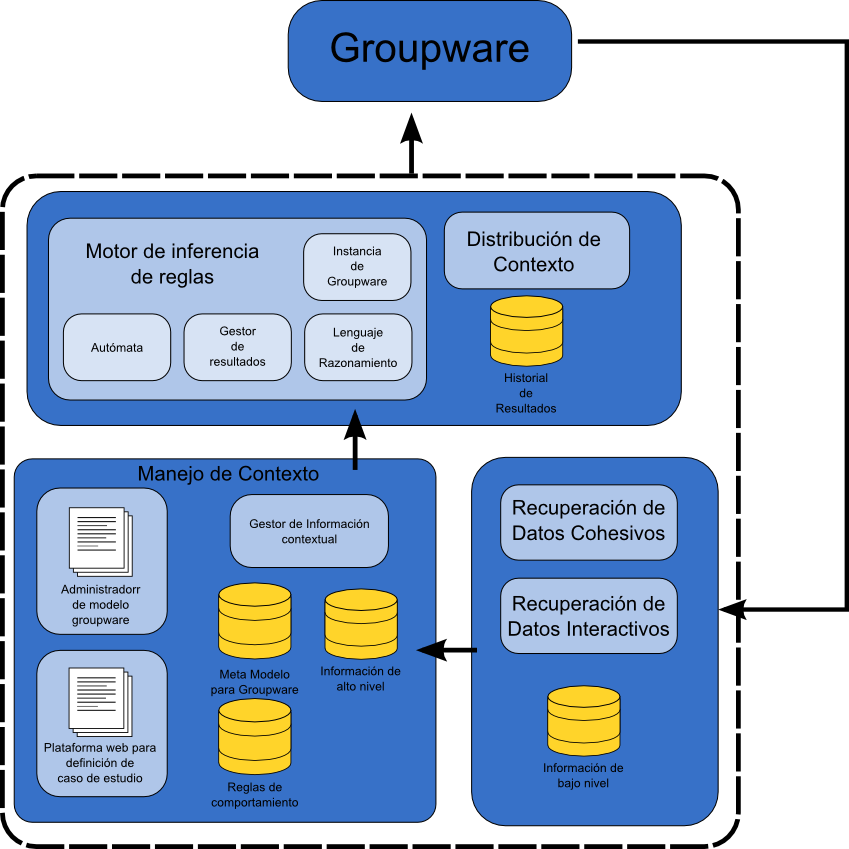
\includegraphics[scale=0.40]{images/arqui2}
\caption{Arquitectura propuesta}
\label{ARCH:propuesta}
\end{figure}

La arquitectura, similar a la arquitectura en que se bas\'o, se divide en tres capas; la capa de recuperaci\'on de datos, la capa de gestion de datos y la capa de uso de contexto. En la primera capa, la de recuperac\'on de datos, se captura informaci\'on contextual enviada por el groupware por medio de servicios web publicados para la comunicaci\'on entre la arquitectura y el sistema, estos datos son enviados en un formato espec\'ifico para que capas superiores puedan procesarla. Seguido de este m\'odulo est\'a el degesti\'on contextual, este gestor se encarga de registrar, actualizar y recuperar la informaci\'on contextual en bases de datos, es a este nivel donde el meta modelo y el modelo del sistema se elaboran y donde los datos enviados desde el groupware se registran y son recuperados para inferir resultados en niveles superiores.

En esta capa se encuentra una plataforma en la que se pueden dar de alta elementos del modelo de actividad. Para poder ingresar al sistema con un caso de estudio, se tiene que dar de alta con un nombre y una contrase\~na para el logueo, esto se lleva a cabo en la vista mostrada en la figura \ref{Ptf:registro}

\begin{figure}
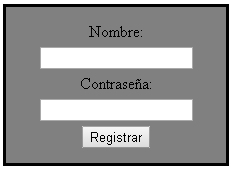
\includegraphics{images/RegistroProto.png}
\caption{Registro de caso de estudio}
\label{Ptf:registro}
\end{figure}

En la figura \ref{Ptf:login} se observa un formulario para le logueo al sistema, esto para poder asociar los elementos a un caso de estudio en espec\'ifico y los elementos est\'en disponibles s\'olo para los casos para los que fueron especificados.

\begin{figure}[h!]
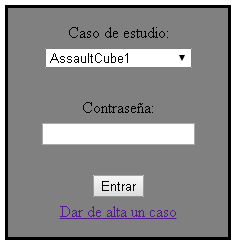
\includegraphics{images/LoginProto.png}
\caption{Login de acceso a la plataforma.}
\label{Ptf:login}
\end{figure}

\begin{figure}[h!]
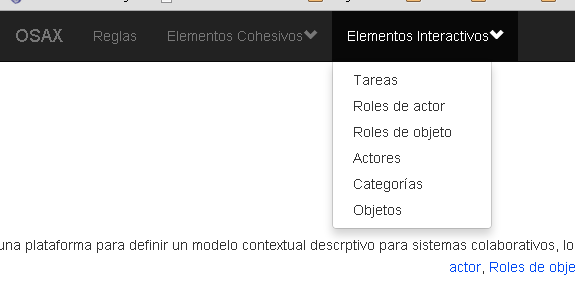
\includegraphics[scale=.6]{images/homeProto.png}
\caption{P\'agina inicial de la plataforma}
\label{Ptf:home}
\end{figure}

\begin{figure}[h!]
\includegraphics{images/TareasPsroto.png}
\caption{Vista de registro de elementos}
\label{Ptf:registro}
\end{figure}

En la \'ultima secci\'on de la arquitectura, uso de contexto, los datos contextuales recuperados son procesados por un motor de inferencia que da como resultado informaci\'on de inter\'es para los usuarios o comandos de ejecuci\'on para la adaptaci\'on del sistema a la situaci\'on actual. El nucleo de este motor es un aut\'omata que especifica un lenguaje para definir reglas, mismas que van a ser definidas en las plataformas antes mencionadas, dentro del motor se har\'a una instancia del modelo del groupware con los datos que env\'ie el sistema, as\'i se puede comparar su estado actual con las reglas de inferencia con el objetivo de ofrecer resultados coherentes al tiempo en el que el sistema se ejecuta. Los resultados obtenidos son gestionados por un administrador de resultados que almacena los datos en una base de datos para mantener registro hist\'orico del comportamiento del groupware. Una vez obtenidos y almacenados los resultados un m\'odulo de distribuci\'on de datos se encarga de enviar la informaci\'on al groupware con la informaci\'on de entrega necesaria. Este proceso es iterativo, ya que vive por el tiempo en el que el groupware opera.

\section{Conclusiones}
Esta arquitectura está diseñada para apoyar el trabajo colaborativo, pero su modelo se puede utlizar para brindar consciencia contexual a otro tipo de sistemas, se implementar\'a en el groupware Assault Cube y se probar\'an sus resultados, con esto se pretende evaluar el desempe\~no de la arquitectura. Har\'ia falta una interfaz acoplable al groupware para que este se pudiera comunicar con la arqutiectura con facilidad. La eficiencia de los resultados depende de las reglas definidas, si las reglas est\'an establecidas para apoyar al grupo de trabjo colaborativo entonces la arquitectura tambi\'en.
 